\chapter{Extensão das funcionalidades}

No capítulo anterior, foi apresentada uma visão geral do sistema e alguns de seus principais componentes. Esse capítulo tem como objetivo descrever as implementações das extensões realizadas no servidor.

As extensões foram realizadas em diferentes componentes da base. Novas tabelas foram adicionadas ao banco de dados para apresentação dos dados em tempo real. Uma nova interface foi acoplada ao servidor e o novo modelo de propagação foi implementado, visando aumentar a acurácia da resposta do servidor referente à quantidade de canais livres no espectro de frequência.

\section{\textit{Frontend} }

O termo \textit{frontend} se refere à camada de apresentação dos dados e interação com o usuário final. No trabalho atual, visando facilitar a interação do usuário com o servidor e exibir as informações presentes na resposta das requisições em um formato mais apresentável, foi implementada uma página Web responsiva, na qual o usuário é capaz, através de um mapa, de consultar a base e obter a quantidade de canais livres. Também é apresentado um mapa de calor representando a distribuição de canais livres em uma porção região sudeste do Brasil.
Para o desenvolvimento da página Web, foi necessário o uso de um conjuno de tecnologias, apresentadas a seguir.

\
\subsection{HTML}

Considerada a linguagem de marcação da World Wide Web ~\cite{htmlw3cs}, o \textit{HyperText Markup Language} (HTML) é a base do \textit{frontend}, servindo como o esqueleto da página. Todas as outras tecnologias implementadas trabalham sobre os elementos inicialmente criados nessa linguagem.

Foi criada pelo físico britânico Tim Berners-Lee, também criador do HTTP,
na década de 90. Inicialmente, Tim tinha a intenção de resolver um problema no laboratório onde trabalhava, o European Organization for Nuclear Research, também chamado de CERN. Diversos artigos científicos citavam outros, que por sua vez citavam outros artigos relacionados. Essa distribuição de conhecimento dificultava o acesso rápido e prático às informações, pois era necessário saber em qual máquina estava armazenado fisicamente determinado artigo para acessá-lo. Além disso, o compartilhamento de artigos deveria ser feito fisicamente, por meio de CDs ou HDs.

Com isso, Tim buscou criar documentos estruturados, baseados em \textit{
tags}, que estariam interconectados. Com isso, bastaria um click para acessar um documento relacionado, formando uma rede de documentos. Surge então, o primeiro protótipo da Web.

Atualmente, o HTML é mantido pela World Wide Web Consortium (W3C) \abbrev{W3C}{World Wide Web Consortion}. Após um longo período sem a publicação de novas versões, sua última versão, visando acompanhar o desenvolvimento da Web nas últimas duas décadas, foi lançado em 2008, o HTML5~\cite{htmlw3cs}.  

Um documento HTML é estruturado por \textit{tags}, de diferentes tipos, cada uma representando o tipo de informação contida entre elas, como: texto puro, imagem e arquivos, entre outros formatos possíveis.


\subsection{JavaScript}

Javascript é uma linguagem de programação dinâmica, amplamente utilizada em conjunto com o documento HTML. Ela é utilizada para dinamizar o funcionamento da página Web, através de scripts que podem ser escritos diretamente no arquivo HTML (Através da \textit{tag script}), ou em arquivos externos, que são importados pelo HTML.

Atualmente, a linguagem é utilizada não só para melhorar a experiência do usuário nas páginas Web, mas como linguagem de programação dos servidores, com o surgimento de tecnologias como Node.js.

\subsection{CSS}

Com o desenvolvimento da Web, notou-se que as \textit{tags} do HTML estavam ficando muito grandes, com muitos atributos, o que acabava dificultando a manutenção do código. Com isso, visando extrair do HTML os parâmetros referentes ao estilo da página, surgiu o Cascading Style Sheets (CSS) ~\abbrev{CSS}{Cascading Style Sheets}, linguagem utilizada na formatação do estilo da página. Atualmente, sua versão é o CSS3, com suporte à animação de elementos do HTML.

\subsection{Implementação}

Com a utilzação das linguagens citadas anteriormente, foi criada uma página Web, onde o usuário é capaz de observar um mapa de calor representando a ocupação das faixas de frequência no intervalo da Tv analógica, e consultar a base para obter em um ponto específico, a quantidade de canais livres e as informações de frequência dos mesmos.


\subsubsection{Estrutura da Página}

Para acessar a página, basta acessar a URL abaixo. Os arquivos com a implementação da página estão presentes na pasta \textit{frontend}, no diretório do servidor.

\begin{itemize}
\item http://servidor/home
\end{itemize}

Ao carregar a página, um mapa é apresentado à direita, e quatro opções à esquerda. Essas opções consistem no modelo a ser exibido. Dentro do mapa, há um marcador que pode ser movido e em seguida uma consulta é enviada ao servidor, passando como parâmetro a localização do marcador e o modelo selecionado. Como resposta, uma lista é apresentada com os canais livres e sua frequência naquela localização.

Para obter o mapa de calor representando o espectro no estado do Rio de Janeiro, foi necessário modificar o servidor. Uma nova URL foi adicionada para realizar o cálculo de canais livres em uma dada região.

Um exemplo de como obter a quantidade de canais livres em um região é ilustrado abaixo. São passados como parâmetros dois pontos, o servidor assume que esses pontos definem a diagonal de um paralelogramo, itera sobre os pontos contidos nesse polígono e retorna um grupo de pontos para o cliente.


\begin{lstlisting}			

http://localhost:8182/SAM/model/1/available/region?lat=-22&lng=-44
&lat2=-20&lng2=-40

\end{lstlisting}

Essa resposta é demorada, pois uma grande quantidade de pontos é processada. Inicialmente, o servidor não persistia nenhum dos cálculos realizados anteriormente, portanto, para cada região especificada, seria necessário recalcular a cada nova consulta. Esse cálculo demorava cerca de duas horas, retornando aproximadamente 40 mil pontos para o estado do Rio de Janeiro.

Visando melhorar a experiência do usuário e poupar processamento no servidor, foi criada uma nova tabela, com os pontos calculados anteriormente. A tabela \textit{available\_channels} possui três colunas: \textit{Latitude}, \textit{Longitude} e \textit{Available\_Channels}. Com isso, o servidor apenas acessa o banco e retorna para o usuário em menos de 1 segundo, os pontos da região especificada pela url, se a mesma já tiver sido processada anteriormente.

\subsubsection{API de mapas}

Inicialmente, utilizou-se a API de mapas da Google, o Google Maps~\cite{googlemaps}. Os pontos foram passados no formato JSON para a página e um \textit{layer} do tipo \textit{heatmap} era adicionado com esses pontos. A visualização não ficou agradável, como mostra as figura \ref{fig:gmaps}.

\begin{figure}[htb]
\centering
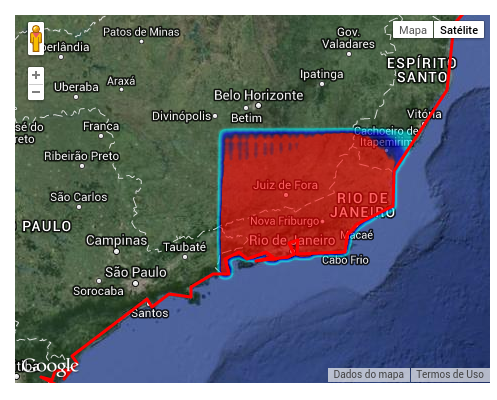
\includegraphics[width=0.8\textwidth]{figs/gmaps}
\caption[Mapa utilizando API da Google.]
{Mapa utilizando API da Google.}
\label{fig:gmaps}
\end{figure} 

A forma com que os pontos são aproximados na redução do zoom não apresenta corretamente a distribuição de canais, perdendo informação.

Visando contornar esse problema, utilizou-se a biblioteca em JavaScript criada por Patrick Wied, a heatmap.js ~\cite{heatmapjs}. Porém, a experiência do usuário ainda ficou ruim, pois a distribuição dos pontos não estava suave, como mostra a figura \ref{fig:heatmapjs}.

\begin{figure}[htb]
\centering
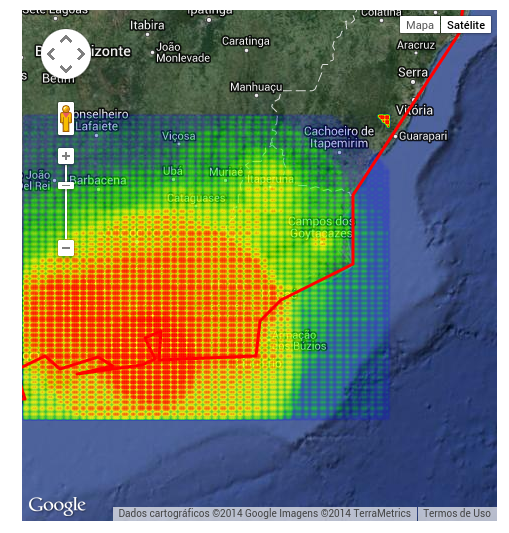
\includegraphics[width=0.8\textwidth]{figs/heatmapjs}
\caption[Mapa utilizando a heatmap.js.]
{Mapa utilizando a heatmap.js.}
\label{fig:heatmapjs}
\end{figure} 

\FloatBarrier

Por fim, utilizou-se a API de mapas criada pela Nokia, HERE ~\cite{heremaps} em conjunto com uma biblioteca em Javascript chamada jHERE~\cite{jhere}. O resultado será apresentado no próximo capítulo.

\section{\textit{Backend}}

\subsection{Servindo a página}

No trabalho realizado anteriormente, o servidor só era acessado via URL e suas respostas vinham no formato XML, o que dificultava a análise dos dados da base. No trabalho atual, para servir a página do \textit{frontend}, foi criado uma nova classe que herda da classe \textit{Application}, presente na biblioteca Restlet~\cite{restlet}. Essa nova classe foi chamada de \textit{HTMLApplication}.

\subsection{Implementação do Longley-Rice}

Para a implementação do Longley-Rice, foi necessário realizar alterações no servidor previamente desenvolvido. 

Foi criada uma nova classe, que herdava de \textit{PropagationModel}, assim como os outros modelos implementados anteriormente~\cite{tccmarcelo}. A nova classe \textit{LongleyRice} implementa os métodos \textit{
interferes()} e \textit{maxDistance()}. O método \textit{maxDistance()} determina o alcance máximo do dispositivo, enquanto o método \textit{interferes()} determina se a soma dos raios dos alcances dos dispositivos primário e secundários supera a distância física entre eles.

\begin{lstlisting}

public double maxDistance(TransmissionDevice dev,
				 TransmissionDevice ant)

\end{lstlisting}

\subsection{Alterações no banco}

Para implementação do modo ponto-a-ponto, era necessário ter informações sobre as elevações do Estado do Rio de Janeiro. Esses dados foram obtidos da Divisão de Sensoriamento Remoto, do Instituto Nacional de Pesquisas Espaciais (INPE)~\cite{elevationdata}.

\begin{figure}[htb]
\centering
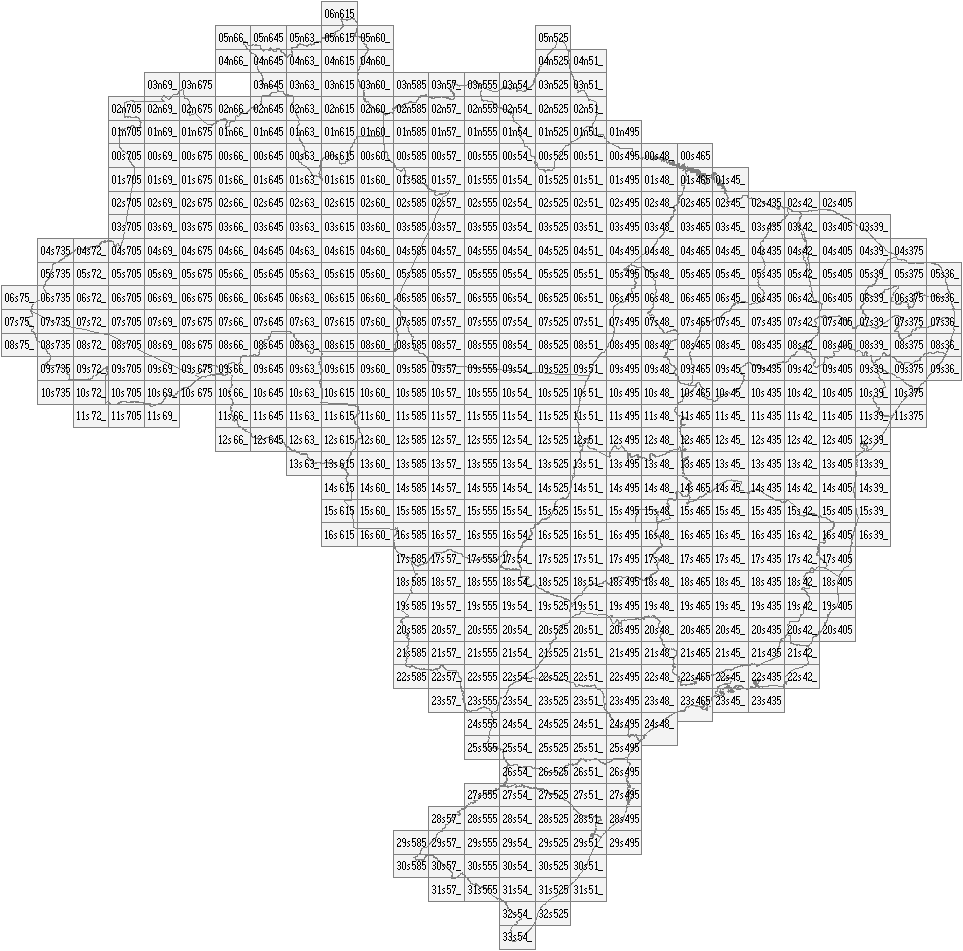
\includegraphics[width=1\textwidth]{figs/elevacaobrasil}
\caption[Elevação do território brasileiro.]
{Elevação do território brasileiro}
\label{fig:elevacaobrasil}
\end{figure}

\FloatBarrier

Esses dados apresentam as elevações presentes no território brasileiro. Estão divididos em quadrantes, cada um com 2.343.600 pontos e suas respectivas elevações. Nesse trabalho, foram utilizados os quadrantes que tinham os dados do estado do Rio de Janeiro, utilizando 7 quadrantes, totalizando 16.405.200 pontos.

Esses pontos foram inseridos em uma tabela denominada ~\textit{elevations}. Por conta do seu tamanho, o tempo de processamento ficou bastante lento e foram necessárias certas adaptações na tabela para melhorar a eficiência das consultas.

As colunas de latitude e longitude foram transformadas em chave primária, pois cada localização é única e com isso o tempo de consulta foi reduzido por conta dos índices criados pelas chaves.